\documentclass[../../main.tex]{subfiles}
    
    \lstset{basicstyle=\small,
      showstringspaces=false,
      commentstyle=\color{black},
      keywordstyle=\color{blue}
    }
    
    \graphicspath{{images/Konzepte/}{../../images/Konzepte/}}


    \begin{document}
    \subsection{Elektronik Komponenten}
    In diesem Kapitel wird der Aufbau der Elektronik des Fahrzeuges beschrieben. \\
    Die Abbildung \ref{fig:et_komponenten} veranschaulicht den Aufbau der Elektronik. Darauf sind alle logischen Verbindungen eingezeichnet. Weitere Elektrische Verbindungen für die Stromversorgung werden im Kapitel \ref{et_stromversorgung} weiter erläutert.\\
    Zentral dabei ist der Mikrocontroller Tiny K22. Die Software auf dem Mikrocontroller initialisiert alle Komponenten, überwacht deren Status und sendet die nötigen Informationen an  das Pi. Diese Schnittstelle ist detailliert im Kapitel \ref{interface_pi_tiny} beschrieben.\\
    Die Schnittstelle über den Debugger zum PC wird hier nicht weiter beschrieben, da diese Verbindung nur zum Entwickeln benutzt wird und für das Endgültige Produkt nicht mehr von bedeutung ist sobald alles funktioniert.

    \begin{figure}[H]
        \centering
        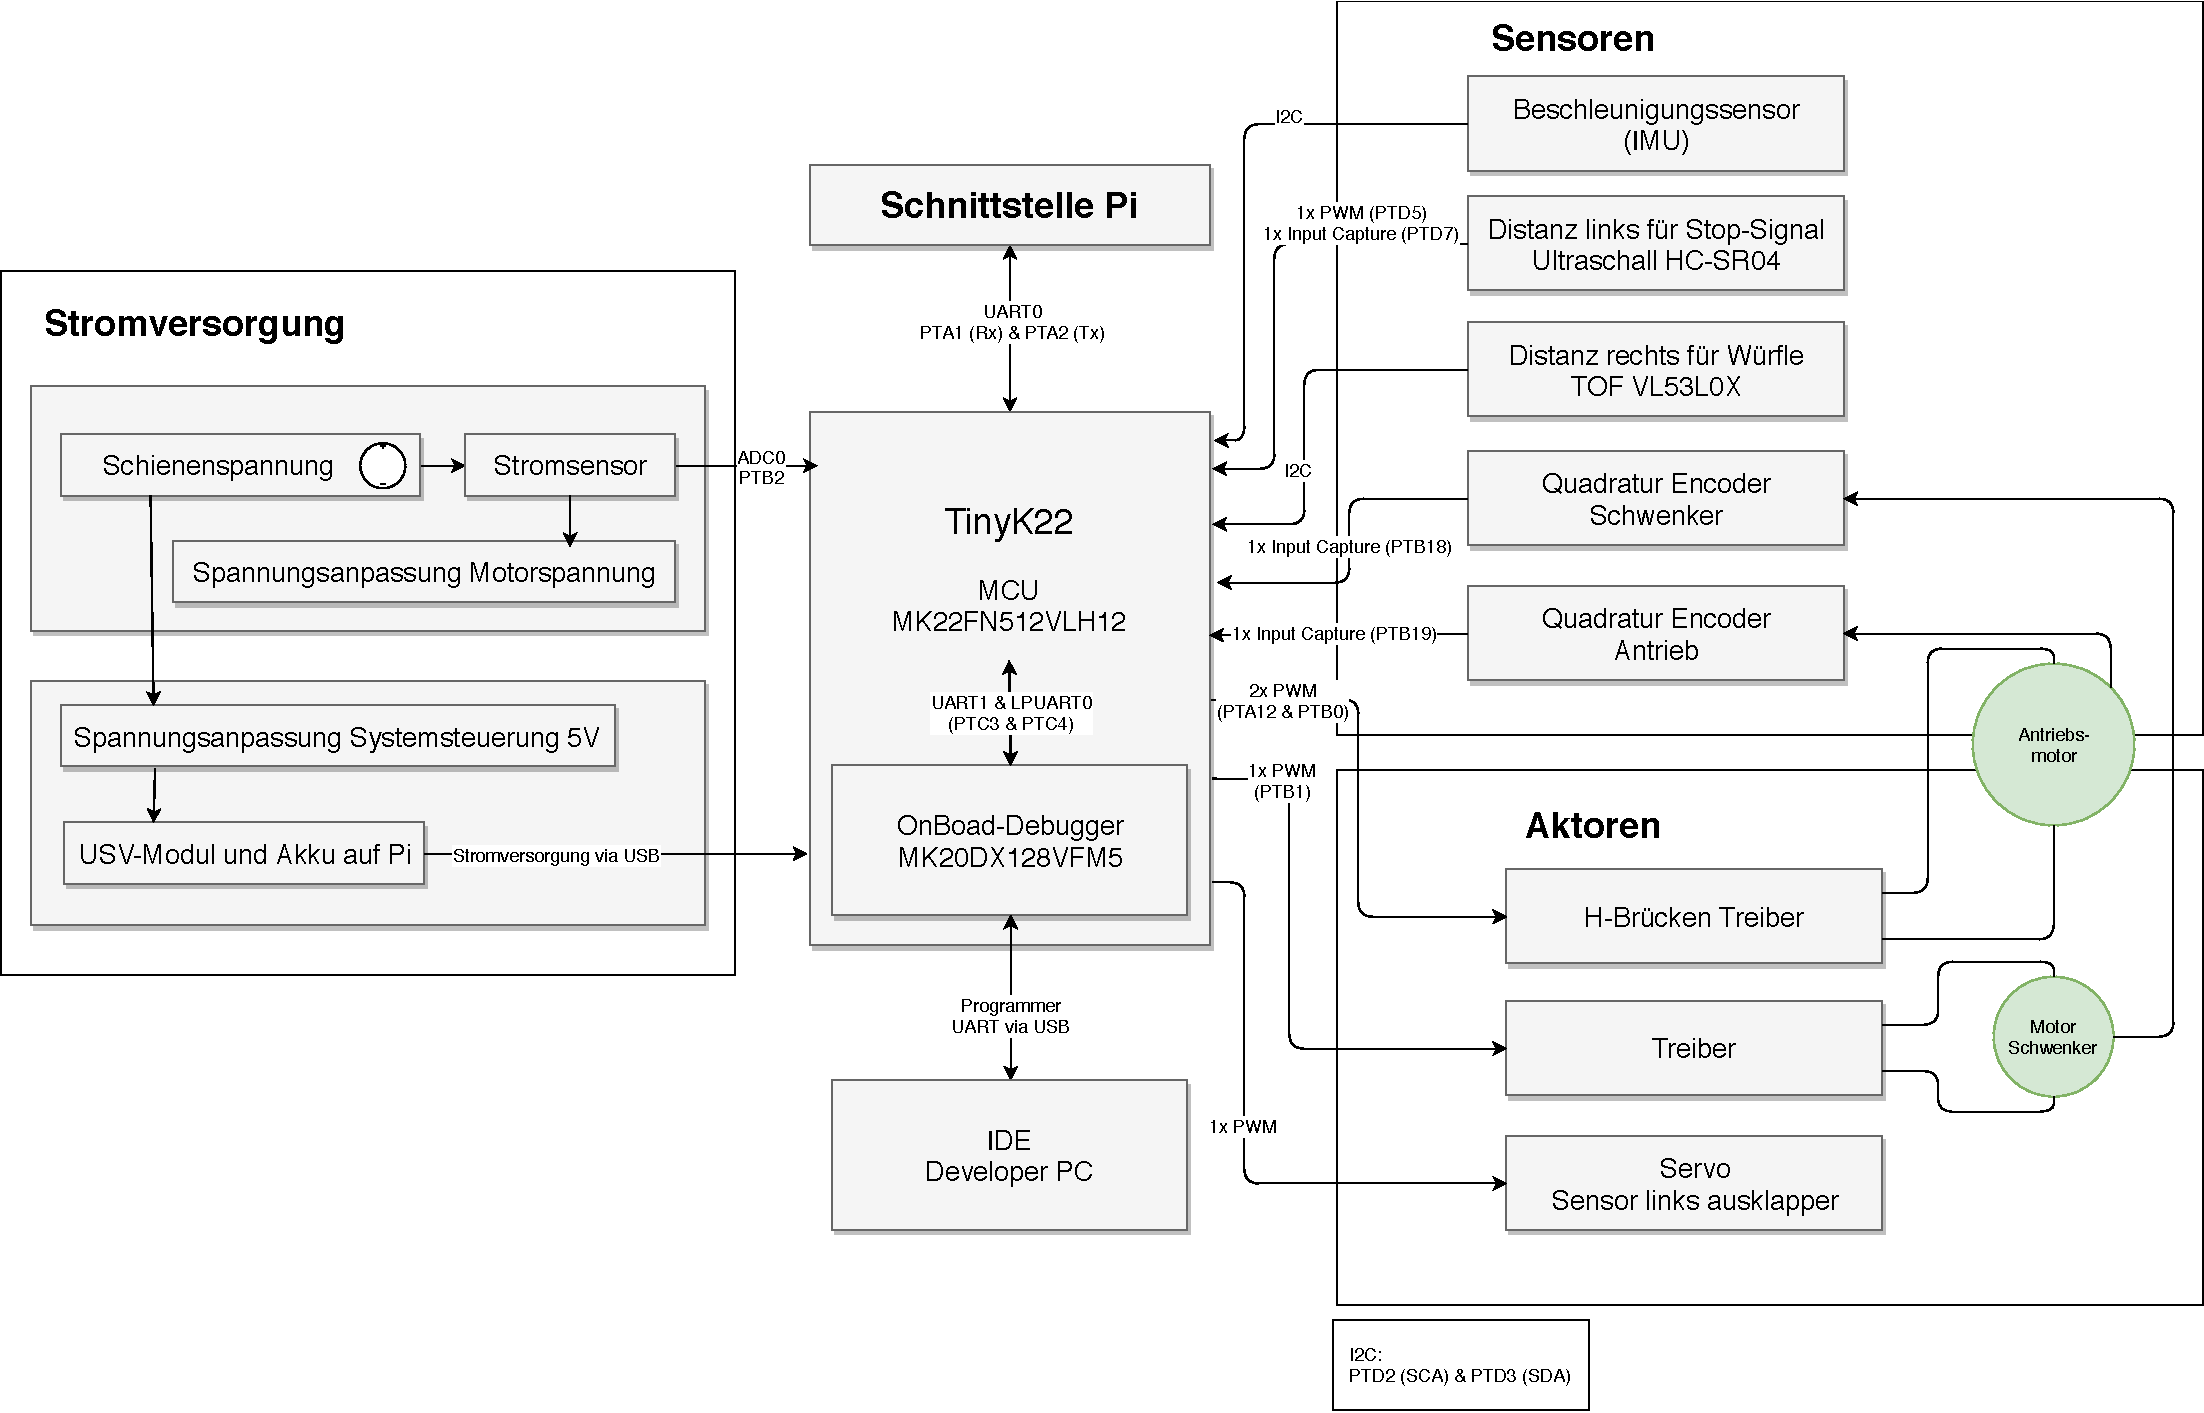
\includegraphics[width=1.0\textwidth]{../../drawings/KomponentenDiagramm/KomponentenDiagramm_ET.pdf}
        \caption {Komponentendiagramm Elektronik}
        \label{fig:et_komponenten}
    \end{figure}

    \subsubsection{Stromversorgung} \label{et_stromversorgung}
    Die Energie für das System wird über die Schienen bezogen.\\ 
    Die Antriebsenergie wird direkt von den Schienen bezogen und lediglich auf die korrektre Motorenspannung angepasst. Die Systemsteuerung wird über ein StromPi 3 mit Strom versorgt. Als Primärstromquelle wird dafür die Schienenspannung benutzt. Bei der Hochgeschwindigkeitsfahrt wird diese Quelle abgeschalten, damit die Gesammte Energie für den Antrieb zur Verfügung steht. Das StromPi schaltet sofort auf die sekundäre Stromversorgung für das Pi. Diese sekundäre Quelle wird durch einen LiFePO4-Akku auf dem StromPi realisiert. Sobald die Primärstromquelle von den Schienen wieder zur Verfügung steht wird der Akku wieder nachgeladen.\\
    Das Pi zero und das TinyK22 mit diversen Sensoren und Aktoren werden über die USB-Anschlüsse des Pi versorgt.

    \textbf{Antriebsenergie}\\
    Die Energie für den Antrieb wird direkt von den Schienen bezogen. Bei der Hochgeschwindigkeitsfahrt werden alle anderen Verbraucher von den Schienen deaktiviert um die gesamte Energie für den Antrieb nutzen zu können.
    
    \textbf{Verpolungsschutz}\\
    Auf den Schienen steht eine Gleichspannung zur Verfügung, wobei eine Schienenseite der $+$ Pol und die andere Seite der $-$ Pol ist. Daraus ergibt sich das Problem, dass beim Platzieren des Zuges entgegen der vorgesehenen Fahrtrichtung eine Verpolung stattfindet. Auch ist die zuordnung der Pole in der Aufgabenstellung noch nicht spezifiziert. Um sicherzustellen, dass das System unabhängig von der Polung der Schienen funktioniert muss eine Gleichrichtung realisiert werden. Dies kann mit einem Brückengleichrichter realisiert werden. (siehe Abbildung \ref{fig:et_bruckengleichrichter})

    \begin{figure}[H]
        \centering
        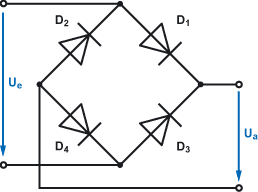
\includegraphics[width=0.3\textwidth]{Brueckengleichrichter.png}
        \caption {Brückengleichrichter \\Quelle: https://www.elektronik-kompendium.de/sites/slt/1807181.htm}
        \label{fig:et_bruckengleichrichter}
    \end{figure}

    Die Ausgangsspannung $U_a$ hat dabei immer dieselbe Polarität, unabhängig welche Polarität $U_e$ hat. \\
    Für den Hochgeschwindigkeitszug wird ein "B40C 3700-2200"  verwendet. Dabei hantelt es sich um eine Integrierte Schaltung für einen Brückengleichrichter. Der maximal zulässige Strom ist dabei $3.7A$. Bei diesem Strom fällt über dem Gleichrichtung eine Spannung von ca $1V$ ab.

    \textbf{Spannungsanpassung}\\
    Gemäss der Aufgabenstellung stehen $20\pm2V$ bei bis zu $3A$ zur Verfügung. Aufgrunde der grossen Toleranz von $4V$ muss die Spannung angepasst werden um eine stabile Spannung zur sicherzustellen. Dafür wird ein DC-DC Converter verwendet. Zu beachten dabei ist, dass der Converter für den maximalen Strom von $3A$ ausgelegt ist.\\

    \textbf{Unterbrechungssicherheit}\\
    Um sicherzustellen, dass ein allfälliger Wackelkontakt der Schleifkontakte überbrückt werden kann und um grössere Spannungsschwankungen zu vermeiden wird ein Kondensator als Stützung eingesetzt.

    \textbf{Stromüberwachung}\\
    Um den Stromverbrauch des Antriebs zu überwachen wie ein Strommesswiderstand eingesetzt. Eine Differenzverstärkerschaltung bereitet die Spannung über dem Strommesswiderstand auf, damit der Mikrocontrollers mit dem Analog-Digital Wandler den Strom bestimmen kann. Mit dieser Information kann die Software des Mikrocontrollers auf Stromspitzen reagieren und z.B. die Geschwindigkeit reduzieren. Der Stromverbrauch ist auch für Entwicklungs- und Testphase eine sehr wertvolle Information, damit das System optimal ausgelegt werden kann.  \\
    Zur Messung wird ein "13FR200E - Strommesswiderstand" verwendet. Dieser hat einen Widerstand von $0.2\Omega$. Der Strom kann daraus mit dem Ohmscheng gesetz bestimmt werden. $$I=\frac{U_R}{R}=\frac{U_R}{0.2\Omega} $$
    \\
    \textbf{Akku}\\
    Während der Hochgeschwindigkeitsfahrt wird die Systemsteuerung wird über einen Akku mit Storm versorgt. Die benötige Leistung der einzelnen Komponenten ist in Tabelle \ref{tab:et_komponente_leistung} aufgeführt. Im schlimmsten Fall soll der Akku das System dabei mindestens für zwei durchläufe mit Energie versorgen können.\\
    Eine Runde darf maximal vier Minuten dauern, das bedeutet die Energie vom Akku muss für mindestens 8 Minuten reichen. Daraus ergibt sich für die Energie $$E=P\cdot t = 14.2W \cdot 8min = 113.6Wmin = 1.9Wh$$

    \begin{table}[H] \centering
        \begin{tabular}{|l|r|}
        \hline
        \textbf{Komponente}     & \textbf{Leistung (max)} \\ \hline
        Raspberry Pi 3 Model B  & 12.50W \nocite{PiShopPi3ModelBp}                 \\ \hline
        Raspberry Pi zero W     & 1.20W \nocite{RaspiTvPiZeroPower}                   \\ \hline
        Tiny K22                & 0.10W \nocite{K22DataSheet}       \\ \hline
        Encoder                 & 0.07W                   \\ \hline
        H-Brückentreiber        & 0.02W                   \\ \hline
        Treiber Schwenker Motor & 0.5mW                   \\ \hline
        Beschleunigungssensor   & 0.3mW                   \\ \hline
        TOF-Sensor              & 20mW                    \\ \hline
        Ultraschall Sensor      & 75mW                    \\ \hline
        \textbf{Total}          & \textbf{14.20W}         \\ \hline
        \end{tabular}
        \caption{benötigte Leistung der Komponenten}
        \label{tab:et_komponente_leistung}
    \end{table}

    Das StormPi Modul wird mit einem LiFePO4-Akku ergänzt. Der Standartakku hat $1000mAh$. Bei einer Spannung von $3.7V$ entspricht dies $3.7Wh$. \\
    Dies ist genügend für zwei durchläufe und da der Akku ausserhalb der Hochgeschwindigkeitsfahrt nachgeladen werden soll, reicht dieser Akku gut.

    \subsubsection{Sensoren} \label{et_sensoren}
    Mit diversen Sensoren sollen folgende Daten aufgenommen werden. Folgende Daten sollen aufgezeichnet werden:
    \begin{itemize}
        \item Beschleunigung
        \item Geschwindigkeit
        \item Position
        \item Distanz rechts (für Erkennung Würfel)
        \item Distanz links (für Erkennung Haltesignal)
    \end{itemize}

    \textbf{Beschleunigung}\\
    Die Beschleunigung wird mit einem Beschleunigungssensor ADXL345 aufgenommen. Dieser kommuniziert über eine $I^2C$ Schnittstelle mit dem Mikrocontrollers. Er liefert jeweils die Beschleunigung in x-, y-, und z-Richtung. Der Sensor wird parallel zur Fahrtrichtung montiert, sodass es reicht eine Beschleunigungsrichtung für die Querbeschleunigung und eine Richtung für die Längsbeschleunigung auszuwerten. Die Verwendung des Sensors ist in Kapitel \ref{pi_beschleunigung} detailliert beschreiben.\\

    \textbf{Geschwindigkeit}\\
    Die Geschwindigkeit wird hauptsächlich über den Quadratur Encoder am Antriebsmotor aufgenommen. Zusätzlich wird die Geschwindigkeit über die Beschleunigung zur Plausibilitätskontrolle nachgerechnet.

    \paragraph{Quadratur Encoder:} Der Quadratur Encoder MR, Typ L gibt 256 Impulse pro Umdrehung. Der Verlauf eines Impulses ist in Abbildung \ref{fig:et_encoder} dargestellt. Der Encoder stellt drei Kanäle zur Verfügung. Über den Kanal $A$ und $B$ kann einzeln die Geschwindigkeit bestimmt werden. Durch auswerten der Phasenverschiebung der beiden Kanäle ("$A$ eilt $B$ vor" oder "$A$ eilt $B$ nach") kann zusätzlich noch die Drehrichtung bestimmt werden. Der Kanal $I$ ist mit Kanal $A$ und $B$ synchronisiert und kann ebenfalls zur Bestimmung der Geschwindigkeit dienen.\\
    Für die Bestimmung der Geschwindigkeit kann die Dauer eines Impulses gemessen werden oder es können die Anzahl Impulse in einer bestimmten Zeit gezählt werden. Für dieses Projekt soll die Dauer des Impulses gemessen werden. Der Vorteil dieser Methode ist die bessere Präzision, da nach jedem einzelnen Impuls die durchschnittliche Geschwindigkeit seit dem letzten Impuls sofort bestimmt werden kann. Das Risiko ist, dass bei hohen Umdrehungszahlen der Mikrocontroller nicht schnell genug ist mit dem Zählen oder dass der Zähler des Mikrocontrollers bei sehr tiefen Umdrehungszahlen überläuft.\\
    Die maximalen Umdrehungszahl des Antriebsmotors liegt bei $8590 min^{-1}$. Mit $256$ Impulsen pro Umdrehung ergibt dies $$8590 min^{-1} \cdot 256 Impulse = 2'199'040 \frac{Impulse}{min}$$.
    Dies sind dann $$ 2'199'040 \frac{Impulse}{min} / 60s = 36'651 \frac{Impulse}{s} $$.
    Dies ergibt eine Impulsdauer von $$\frac{1}{36'651 \frac{Impulse}{s}} = 27.26\mu s$$. Bei der schnellsten möglichen Timer Einstellung auf dem TinyK22 ($60MHz$) ergibt dies noch $1'637 \frac{Ticks}{Impuls}$. Dies ist ein plausibler Wert. Bei der Implementation muss jedoch beachtet werden, dass bei hoher Geschwindigkeit möglichst wenig Zeit in der Interrupt routine verbracht wird, da diese dann sehr of aufgerufen wird.\\
    Damit der Timer nicht überläuft muss der Impuls fertig sein, bevor der Timer den Wert $$2^{32} \approx 4.29 Mrd$$ erreicht wird. Dies ergibt bei $60MHz$ eine Zeit von $$2^{32} \cdot \frac{1}{60MHz} = 71.58s$$. Also ist ein tiefe Umdrehungszahl bis zu $$\frac{1}{71.58s \cdot 256} = 54.6 \cdot 10^{-6} s^{-1} \hat{=} 909 \cdot 10^{-9} min^{-1}$$
    Also sollte diese Umdrehungszahl nicht unterschritten werden. 
    
    \begin{figure}[H]
        \centering
        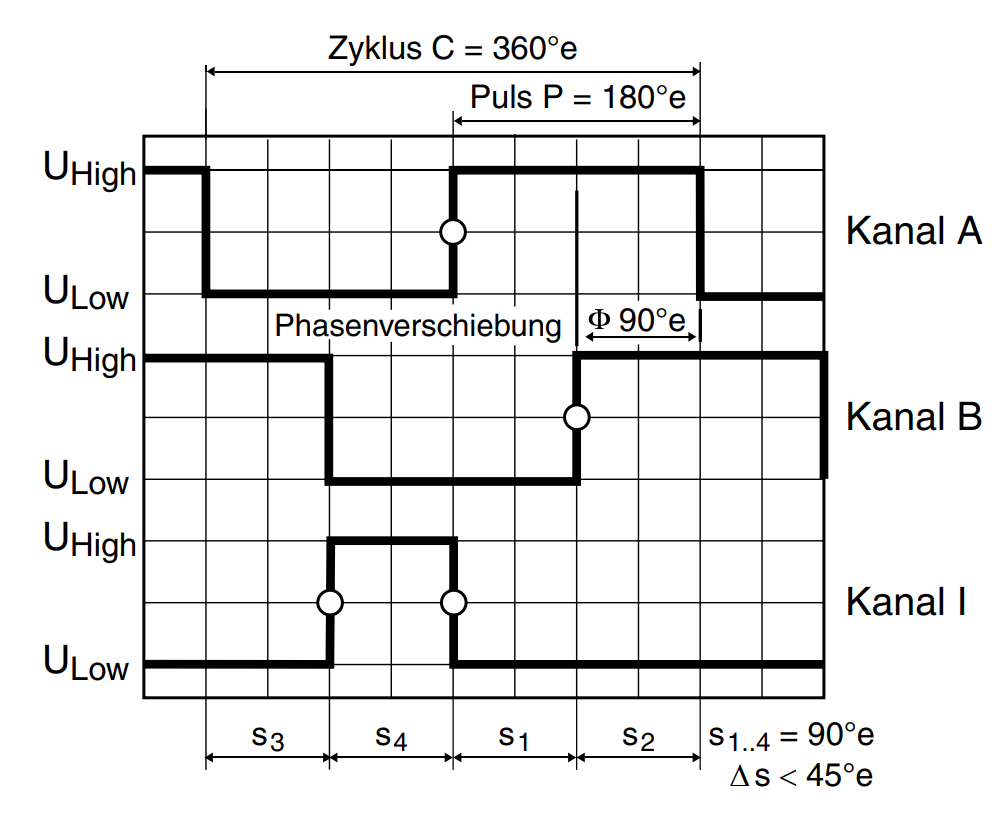
\includegraphics[width=0.8\textwidth]{Encoder_MR.png}
        \caption {Signalverlauf Encoder \\Quelle: Katalogseite 420, Encoder MR Typ L, maxon sensor}
        \label{fig:et_encoder}
    \end{figure}

    Die Geschwindigkeit kann daraus mittels der Mechanischen Übersetzung berechnet werden. 
    \textcolor{red}{TODO: Mechis --> Übersetzun vom Motor auf die Schienen, also $$v_{Zug}(Umdrehungszahl_{Motor}) = ???$$}\\

    \paragraph{Nachrechnen der Geschwindigkeit:}
    Unter der Annahme, dass zu beginn der Messung zum Zeitpunkt $t = 0$ die Geschwindigkeit $0$ ist $(v(t=0) = 0)$ kann die Geschwindigkeit zum Zeitpunkt $t$ bestimmt werden mit $$v(t) = \int_{0}^{t} a(x) dx$$.\\
    Da aber auf einem Digitalen System die Daten nur zu diskreten Zeitpunkten ausgewertet werden können ergibt sich dann eine Summen der Beschleunigungen zum Zeitpunkt $k$ $$v[k] = \sum_{i=0}^{k}a[i] \Delta t$$ 

    \textbf{Position}\\
    Über den Beschleunigungssensor kann man die aktuelle Position auf der Fahrbahn berechnen. Die zurückgelegte Strecke errechnet sich durch Integration der Geschwindigkeit oder durch zweifache Integration der Beschleunigung.\\
    Unter der Annahme, dass zu beginn der Messung zum Zeitpunkt $t = 0$ die zurückgelegte Strecke $0$ ist $(s(t=0) = 0)$ kann die Geschwindigkeit zum Zeitpunkt $t$ bestimmt werden mit $$s(t) = \int_{0}^{t} v(x) dx$$.\\
    Da aber auf einem Digitalen System die Daten nur zu diskreten Zeitpunkten ausgewertet werden können ergibt sich dann eine Summen der Geschwindigkeiten zum Zeitpunkt $k$ $$s[k] = \sum_{i=0}^{k}v[i] \Delta t$$\\
    Die Geschwindigkeit wird gemäss der Beschreibung oben bestimmt.

    \textbf{Distanz}\\
    Auf beiden Seiten des Zuges wird eine Distanzmessung benötigt. Auf der rechten Seite des Zuges muss der Würfel erkennt werden und auf der Linken Seite soll ein ausklappbarer Sensor am Schluss die genaue Distanz zum Haltesignal bestimmen.

    \paragraph{Würfelerkennung:}
    Gemäss der Aufgabenstellung befindet sich der Würfel in einem Abstand von $8\pm1cm$ von der Gleismitte. Somit muss der Distanzsensor Distanzen zwischen ca. $20mm$ und $80mm$ erkennen können. Der exakte Wert der Distanz ist dabei nicht entscheidend, da nur ein bestimmter Schwellwert erkennt werden muss. Die Distanz zum Würfle wird mit einem TOF (Timo-Of-Flight) Sensor VL53L0X ermittelt.

    \paragraph{Haltesignalerkennung:}
    Um möglichst präzise anhalten zu können muss die Systemsteuerung den exakten Wert der Distanz zum Haltesignal kennen. Dies wird mit einem Distanzsensor ermittelt. Diese Distanz wird mit einem Ultraschall Sensor HC-SR04 gemessen. Es ist entscheidend, dass der Sensor korrekt und mit wenig Toleranz auf der Mechanik befestigt wird um eine exakte Ausrichtung auf das Haltesignal sicherzustellen.
    
    \subsubsection{Aktoren}
    Die Aktoren stellen die Schnittstelle zur Mechanik dar. Diese sollen alle nötigen Mechanischen bewegungen auf Befehl des Mikrocontrollers ausführen.\\

    \textbf{H-Brücken Treiber für Antriebsmotor}\\
    Um den Antriebsmotor anzusteuern wird ein H-Brückentreiber verwendet. Damit kann der Motor durch ein PWM Signal in der Geschwindigkeit fast beliebig eingestellt werden. Über die wahlweise Ansteuer einer der beiden eingänge der H-Brücke wird die Richtung bestimmt.\\
    Es wird ein Arduion IBT\_2 DC-Motoren Treiber mit einem BTS7960 eingesetzt. Dieses Bauteil kann Motoren mit einem Strom von bis zu 43A versorgen. \\
    
    \textbf{Antriebsmotor}\\
    Als Antriebsmotor dient ein Maxon DCX 32 L. Dieser kann eine Leistung von bis zu 70 Watt umsetzen. Dabei zu beachten ist, dass der Anlaufstrom bis zu $70A$ betragen kann. Dieser Strom muss begrenzt werden indem der Mikrocontrollers die Beschleunigung gemäss dem gemessenen Stromverbrach anpasst.\cite{MaxonDCX32L} Dies ist bei einer Versorgungsspannung von 24V spezifiziert. Da aber nicht die maximale Drehzahl benötigt wird kann auch eine entsprechend tiefere Spannung angelegt werden.\\ 

    \textbf{Motorentreiber für Schwenker-Motor}\\
    Da die Richtung immer dieselbe ist reicht für den Schwenker ein normaler DC-Motoren Treiber. Um eine sanfte Beschleunigung und Abbremsung der konstruktion zu ermöglichen, soll auch der Schwenkermotor mit einem PWM angesteuert werden. Als Treiber wird ein Board mit einem L298N verwendet.\\

    \textbf{Schwenkermotor}\\
    Für den Schwenker wir ein Maxon DCX 19 S verwendet. Um die Position des Schwenkers zu bestimmen ist auch an diesem Motor ein Encoder befestigt. Durch die Bestimmung der nötigen Umdrehungen bis der Schwenker eingefahren ist kann genau festgestellt werden wie viele Impulse abgewartet werden müssen bis der Der Motor anhalten muss. \cite{MaxonDCX19S}\\

    \textbf{Distanzsensor links ausklappen}\\
    Um den Sensor beim Parkieren ausklappen zu können wird er an einem Servo befestigt. Sobald die Systemsteuerung entscheidend, dass das korrekte Haltesignal das nächste ist gibt sie den Befehlt den Sensor auszuklappen. Dafür wird ein "Tower Pro Micro Servo SG90" verwendet. Dieser hat ein Drehmoment von bis zu $2.5 kg-cm$. \cite{SG90Datasheet}\\

    \end{document}